% \documentclass[handout]{beamer}
\documentclass{beamer}

\mode<presentation>
{
  \usetheme{default}
  \usefonttheme[onlymath]{serif}
  % \usetheme{Singapore}
  % \usetheme{Warsaw}
  % \usetheme{Malmoe}
  % \useinnertheme{circles}
  % \useoutertheme{infolines}
  % \useinnertheme{rounded}

  \setbeamercovered{transparent=100}
}

\usepackage[english]{babel}
\usepackage[latin1]{inputenc}
\usepackage{alltt,listings,multirow,ulem,siunitx}
\usepackage[absolute,overlay]{textpos}
\TPGrid{1}{1}
\usepackage{pdfpages}
\usepackage{multimedia}
\usepackage{multicol}
\newcommand\hmmax{0}
\newcommand\bmmax{0}
\usepackage{bm}
\usepackage{comment}
\usepackage{subcaption}

% font definitions, try \usepackage{ae} instead of the following
% three lines if you don't like this look
\usepackage{mathptmx}
\usepackage[scaled=.90]{helvet}
% \usepackage{courier}
\usepackage[T1]{fontenc}
\usepackage{tikz}
\usetikzlibrary{decorations.pathreplacing}
\usetikzlibrary{shadows,arrows,shapes.misc,shapes.arrows,shapes.multipart,arrows,decorations.pathmorphing,backgrounds,positioning,fit,petri,calc,shadows,chains,matrix}


% \usepackage{pgfpages}
% \pgfpagesuselayout{4 on 1}[a4paper,landscape,border shrink=5mm]

\usepackage{JedMacros}

\newcommand{\timeR}{t_{\mathrm{R}}}
\newcommand{\timeW}{t_{\mathrm{W}}}
\newcommand{\mglevel}{\ensuremath{\ell}}
\newcommand{\mglevelcp}{\ensuremath{\mglevel_{\mathrm{cp}}}}
\newcommand{\mglevelcoarse}{\ensuremath{\mglevel_{\mathrm{coarse}}}}
\newcommand{\mglevelfine}{\ensuremath{\mglevel_{\mathrm{fine}}}}

%solution and residual
\newcommand{\vx}{\ensuremath{x}}
\newcommand{\vc}{\ensuremath{\hat{x}}}
\newcommand{\vr}{\ensuremath{r}}
\newcommand{\vb}{\ensuremath{b}}

%operators
\newcommand{\vA}{\ensuremath{A}}
\newcommand{\vP}{\ensuremath{I_H^h}}
\newcommand{\vS}{\ensuremath{S}}
\newcommand{\vR}{\ensuremath{I_h^H}}
\newcommand{\vI}{\ensuremath{\hat I_h^H}}
\newcommand{\vV}{\ensuremath{\mathbf{V}}}
\newcommand{\vF}{\ensuremath{F}}
\newcommand{\vtau}{\ensuremath{\mathbf{\tau}}}


\title{Exploiting structure in numerical libraries (PETSc)}
\author{Shrirang Abhyankar, Mark Adams (LBL), Satish Balay, {\bf Jed Brown}, Peter Brune, Emil Constantinescu, Debojyoti Ghosh, Dmitry Karpeev, Matt Knepley (UChicago), Lois Curfman McInnes, Barry Smith, Hong Zhang}

% - Use the \inst command only if there are several affiliations.
% - Keep it simple, no one is interested in your street address.
\institute
{
  {Mathematics and Computer Science Division, Argonne National Laboratory}
}

\date{ANL, 2013-06-18}

% This is only inserted into the PDF information catalog. Can be left
% out.
\subject{Talks}


% If you have a file called "university-logo-filename.xxx", where xxx
% is a graphic format that can be processed by latex or pdflatex,
% resp., then you can add a logo as follows:

% \pgfdeclareimage[height=0.5cm]{university-logo}{university-logo-filename}
% \logo{\pgfuseimage{university-logo}}



% Delete this, if you do not want the table of contents to pop up at
% the beginning of each subsection:
% \AtBeginSubsection[]
% {
% \begin{frame}<beamer>
%   \frametitle{Outline}
%   \tableofcontents[currentsection,currentsubsection]
% \end{frame}
% }

\AtBeginSection[]
{
  \begin{frame}<beamer>
    \frametitle{Outline}
    \tableofcontents[currentsection]
  \end{frame}
}

% If you wish to uncover everything in a step-wise fashion, uncomment
% the following command:

% \beamerdefaultoverlayspecification{<+->}

\begin{document}
\lstset{language=C}
\normalem

\begin{frame}
  \titlepage
\end{frame}

\begin{frame}{From natural structure to efficient algorithms}
  \begin{itemize}
  \item Fluids, structures, plasma, chemistry, mesoscale materials, \ldots
  \item Conservation of mass, energy, \ldots
  \item Approximately balanced dynamics: weather systems, resonance
  \item Design accurate numerical methods that preserve compatibility
  \item Design efficient, scalable algorithms for solving associated algebraic problems
  \end{itemize}
  \begin{center}
    \includegraphics[width=0.8\textwidth]{figures/LaetiRifting}
  \end{center}
\end{frame}

\begin{frame}{Structure is also needed for analysis of models}
  \large
  \begin{itemize}
  \item Optimization
    \begin{itemize}
    \item Smoothness
    \item Convexity
    \item Computability of gradients
    \end{itemize}
  \item Data assimilation and experimental design
    \begin{itemize}
    \item High-dimensional probability distributions
    \item Sparsity of observations
    \end{itemize}
  \item Stability analysis (bifurcations)
  \end{itemize}
\end{frame}

\begin{frame}{PETSc's Goal}
  \Large
  Make the best possible structure-exploiting methods:
  \begin{itemize}
  \item reusable
  \item easy to use
  \item extensible
  \item composable
  \end{itemize}
\end{frame}

\begin{frame}{Scalability definitions}
  \begin{columns}
    \begin{column}{0.5\textwidth}
      {\large Strong scalability}
      \begin{itemize}
      \item Fixed problem size
      \item execution time $T$ inversely proportional to number of processors $p$
      \end{itemize}
    \end{column}
    \begin{column}{0.5\textwidth}
      \includegraphics[width=\textwidth]{figures/KeyesStrongScaling.png}
    \end{column}
  \end{columns}

  \begin{columns}
    \begin{column}{0.5\textwidth}
      {\large Weak scalability}
      \begin{itemize}
      \item Fixed problem size per processor
      \item execution time constant as problem size increases
      \end{itemize}
    \end{column}
    \begin{column}{0.5\textwidth}
      \includegraphics[width=\textwidth]{figures/KeyesWeakScaling.png}
    \end{column}
  \end{columns}
\end{frame}


\begin{frame}[fragile]
  \frametitle{Full Multigrid(FMG)}
  \begin{figure}
  \centering
  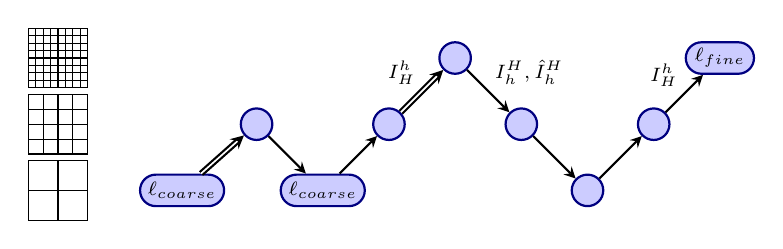
\begin{tikzpicture}
    [>=stealth,
    every node/.style={inner sep=2pt},
    restrict/.style={thick},
    prolong/.style={thick},
    mglevel/.style={rounded rectangle,draw=blue!50!black,fill=blue!20,thick,minimum size=4mm},
    ]
    \begin{scope}\scriptsize
      \newcommand\mgdx{3.0em}
      \newcommand\mgdy{3.0em}
      \newcommand\mgl[1]{(pow(2,#1+1))}
      \newcommand\mgloc[4]{(#1 + #4*\mgdx*#3,#2 + \mgdy*#3)}

      \node[mglevel] (coarseinit) at \mgloc{-3}{0}{0}{0} {$\mglevel_{coarse}$};

      \node[mglevel] (afine) at \mgloc{0}{0}{1}{1} {};

      \node[mglevel] (bcoarse) at \mgloc{2*\mgdx}{0}{0}{1} {$\mglevel_{coarse}$};
      \node[mglevel] (bup1) at \mgloc{2*\mgdx}{0}{1}{1} {};
      \node[mglevel] (bfine) at \mgloc{2*\mgdx}{0}{2}{1} {};

      \node[mglevel] (cdown1) at \mgloc{6*\mgdx}{0}{1}{-1} {};
      \node[mglevel] (ccoarse) at \mgloc{6*\mgdx}{0}{0}{-1} {};
      \node[mglevel] (cup1) at \mgloc{6*\mgdx}{0}{1}{1} {};
      \node[mglevel] (cfine) at \mgloc{6*\mgdx}{0}{2}{1} {$\mglevel_{fine}$};


      \draw[->,restrict,double]
                         (coarseinit) -- node [above right] {} (afine);
      \draw[->,restrict]
                         (afine) -- node [above right] {} (bcoarse);
      \draw[->,restrict]
                         (bcoarse) -- node [above right] {} (bup1);
      \draw[->,restrict,double]
                         (bup1) -- node [above left] {$\mathbb I_H^h$} (bfine);
      \draw[->,restrict]
                         (bfine) -- node [above right] {$I_h^H,\hat I_h^H$} (cdown1);
      \draw[->,restrict]
                         (cdown1) -- node [above right] {} (ccoarse);
      \draw[->,restrict]
                         (ccoarse) -- node [above right] {} (cup1);
      \draw[->,restrict]
                         (cup1) -- node [above left] {$I_H^h$} (cfine);

      %grids
      \newcommand\mghx{0.9*\mgdx}
      \newcommand\mghy{0.9*\mgdy}

      \draw[shift=\mgloc{-2*\mgdx}{0}{2}{0},
      xstep=\mghy/\mgl{2},
      ystep=\mghy/\mgl{2}]
      (-0.5*\mghy,-0.5*\mghy) grid (0.5*\mghy,0.5*\mghy);

      \draw[shift=\mgloc{-2*\mgdx}{0}{1}{0},
      xstep=\mghy/\mgl{1},
      ystep=\mghy/\mgl{1}]
      (-0.5*\mghy,-0.5*\mghy) grid (0.5*\mghy,0.5*\mghy);

      \draw[shift=\mgloc{-2*\mgdx}{0}{0}{0},
      xstep=\mghy/\mgl{0},
      ystep=\mghy/\mgl{0}]
      (-0.5*\mghy,-0.5*\mghy) grid (0.5*\mghy,0.5*\mghy);

  \end{scope}
\end{tikzpicture}
\label{fig:FMG}
\end{figure}
\begin{itemize}
  \item start with coarse grid
  \item $\vx$ is prolonged using $\mathbb{I}_H^h$ on first visit to each finer level
  \item truncation error within one cycle
  \item about five work units for many problems
  \item highly efficient solution method
\end{itemize}
\end{frame}

% \begin{frame}{Hardware Arithmetic Intensity}
  \begin{tabular}{lc}
    \toprule
    Operation                         & Arithmetic Intensity (flops/B) \\
    \midrule
    Sparse matrix-vector product      & 1/6                  \\
    Dense matrix-vector product       & 1/4                  \\
    Unassembled matrix-vector product & $\approx 8$          \\
    High-order residual evaluation    & $> 5$                \\
    \bottomrule
  \end{tabular}

  \bigskip

  \begin{tabular}{lrrr}
    \toprule
    Processor & BW (GB/s) & Peak (GF/s) & Balanced AI (F/B) \\
    \midrule
    E5-2670 8-core      & 35   & 166  & 4.7 \\
    Magny Cours 16-core & 49   & 281  & 5.7 \\
    Blue Gene/Q node    & 43   & 205  & 4.8 \\
    Tesla M2090         & 120  & 665  & 5.5 \\
    Kepler K20Xm        & 160 & 1310 & 8.2 \\ % http://www.elekslabs.com/2012/11/nvidia-tesla-k20-benchmark-facts.html
    Xeon Phi            & 150 & 1248 & 8.3 \\
    \bottomrule
  \end{tabular}
\end{frame}


% \begin{frame}{This is a dead end}
%   \begin{itemize}
%   \item Arithmetic intensity $< 1/4$
%   \item Idea: multiple right hand sides
%     \begin{equation*}
%       \frac{(2 k \text{ flops})(\text{bandwidth})}{\texttt{sizeof(Scalar)} + \texttt{sizeof(Int)}}, \quad k \ll \text{avg. nz/row}
%     \end{equation*}
%   \item Problem: popular algorithms have nested data dependencies
%     \begin{itemize}
%     \item Time step \\
%       \qquad Nonlinear solve \\
%       \qquad \qquad Krylov solve \\
%       \qquad \qquad \qquad Preconditioner/sparse matrix
%     \end{itemize}
%   \item Cannot parallelize/vectorize these nested loops
%   \item<2> \alert{Can we create new algorithms to reorder/fuse loops?}
%     \begin{itemize}
%     \item Reduce latency-sensitivity for communication
%     \item Reduce memory bandwidth (reuse matrix)
%     \item Implicit Runge-Kutta, creates tensor product structure
%     \item Full space/one-shot methods for PDE-constrained optimization
%     \end{itemize}
%   \end{itemize}
% \end{frame}

\begin{frame}{$\tau$ corrections}
  \begin{figure}
  \centering
  \begin{subfigure}[b]{0.18\textwidth}
    \includegraphics[width=\textwidth]{figures/MG/ElasticityCompressTrim}
    %\caption{Initial solution.}\label{fig:elast-initial}
  \end{subfigure} ~
  \begin{subfigure}[b]{0.18\textwidth}
    \includegraphics[width=\textwidth]{figures/MG/ElasticityCompressShearTrim}
    %\caption{Increment.}\label{fig:elast-increment}
  \end{subfigure} ~
  \begin{subfigure}[b]{0.28\textwidth}
    \includegraphics[width=\textwidth]{figures/MG/ElasticityCompressErrorNoTauTrim}
    %\caption{Smoothed error without $\tau$.}\label{fig:elast-error-notau}
  \end{subfigure} ~
  \begin{subfigure}[b]{0.28\textwidth}
    \includegraphics[width=\textwidth]{figures/MG/ElasticityCompressErrorTauTrim}
    %\caption{Smoothed error with $\tau$.}\label{fig:elast-error-tau}
  \end{subfigure}
  \begin{itemize}
  \item Plane strain elasticity, $E=1000,\nu=0.4$ inclusions in $E=1,\nu=0.2$ material, coarsen by $3^2$.
  \item Solve initial problem everywhere and compute $\tau_h^H = A^H \hat I_h^H u^h - I_h^H A^h u^h$
  \item Change boundary conditions and solve FAS coarse problem
    \begin{equation*}
      N^H \acute u^H = \underbrace{I_h^H \acute f^h}_{\acute f^H} + \underbrace{N^H \hat I_h^H \tilde u^h - I_h^H N^h \tilde u^h}_{\tau_h^H}
    \end{equation*}
  \item Prolong, post-smooth, compute error $e^h = \acute u^h - (N^h)^{-1} \acute f^h$
  \item<2> \alert{Coarse grid \emph{with $\tau$} is nearly $10\times$ better accuracy}
  \end{itemize}
  % \caption{Plane strain elasticity, $E=1000,\nu=0.4$ inclusions in $E=1,\nu=0.2$ material.  2-level multigrid with coarsening factor of $3^2$.
  %   Panes (a) and (b) show the deformed body colored by strain.
  %   The initial problem of compression by 0.2 from the right is solved (a) and $\tau = A^H \hat I_h^H u^h - I_h^H A^h u^h$ is computed.
  %   Then a shear increment of 0.1 in the $y$ direction is added to the boundary condition, and the coarse-level problem is resolved, interpolated to the fine-grid, and a post-smoother is applied.
  %   When the coarse problem is solved without a $\tau$ correction (c), the displacement error is nearly $10\times$ larger than when $\tau$ is included in the right hand side of the coarse problem (d).
  % }\label{fig:tau-valid}
  % ./ex49 -mx 90 -my 90 -da_refine_x 3 -da_refine_y 3 -elas_ksp_converged_reason -elas_ksp_rtol 1e-8 -no_view -c_str 3 -sponge_E0 1 -sponge_E1 1e3 -sponge_nu0 0.4 -sponge_nu1 0.2 -sponge_t 3 -sponge_w 9 -u_o vtk:ex49_sol.vts -use_nonsymbc -elas_pc_type mg -elas_pc_mg_levels 2 -elas_pc_mg_galerkin -tau1_o vtk:ex49_tau1.vts -tau2_o vtk:ex49_tau2.vts -taudiff_o vtk:ex49_taudiff.vts -u2_o vtk:ex49_sol2.vts -u2c_o vtk:ex49_sol2c.vts -u3_o vtk:ex49_sol3.vts -u4_o vtk:ex49_sol4.vts -u2err_o vtk:ex49_sol2err.vts -u3err_o vtk:ex49_sol3err.vts -u3c_o vtk:ex49_sol3c.vts -tau3_o vtk:ex49_tau3.vts
\end{figure}
\end{frame}

\begin{frame}{The Great Solver Schism: Monolithic or Split?}
  \begin{columns}
    \begin{column}{0.5\textwidth}
      \begin{block}{Monolithic}
        \begin{itemize}
        \item Direct solvers
        \item Coupled Schwarz
        \item Coupled Neumann-Neumann \\
          (need unassembled matrices)
        \item Coupled multigrid
        \item[X] Need to understand local spectral and compatibility properties of the coupled system
        \end{itemize}
      \end{block}
    \end{column}
    \begin{column}{0.5\textwidth}
      \begin{block}{Split}
        \begin{itemize}
        \item Physics-split Schwarz \\
          (based on relaxation)
        \item Physics-split Schur \\
          (based on factorization)
          \begin{itemize}
          \item  approximate commutators \\
            SIMPLE, PCD, LSC
          \item segregated smoothers
          \item Augmented Lagrangian
          \item ``parabolization'' for stiff waves
          \end{itemize}
        \item[X] Need to understand global coupling strengths
        \end{itemize}
      \end{block}
    \end{column}
  \end{columns}
  \begin{itemize}
  \item Preferred data structures depend on which method is used.
  \item Interplay with geometric multigrid.
  \end{itemize}
\end{frame}


\begin{frame}{Why is exploiting structure hard?}
  \begin{itemize}
  \item Black box interfaces tend to exploit only one or two types of structure at a time
  \item Cutting-edge science often needs to exploit \alert{all} available structure
  \item Generic data structures not well matched to evolving hardware
    \begin{itemize}
    \item More concurrency, less memory per thread
    \item Deeper memory hierarchy, heterogeneous execution
    \end{itemize}
  \item Nonlinearity and coupling with other physical models can change the available structure
  \item Assumptions break down between model problems and production
  \item Assumptions fall through the cracks
    \begin{itemize}
    \item E.g., model nonlinearity breaks assumption of Gaussian probability distribution
    \item Switching to more ``robust'' method makes problem intractable
    \end{itemize}
  \item Applications seek to satisfy disparate user groups, make assumptions invalid in other contexts
  \end{itemize}
\end{frame}

\end{document}
